\documentclass[11pt]{article}
\usepackage[utf8]{inputenc}
\usepackage{lingmacros}
\usepackage{tree-dvips}
\usepackage{enumitem}
\usepackage{graphicx}
\usepackage{lmodern}
\usepackage[T1]{fontenc}
\usepackage[bottom]{footmisc}
\graphicspath{ {./images/} }

\newenvironment{remerciements}
  {
   \thispagestyle{empty}% no header and footer
   \vspace*{\stretch{1}}% some space at the top
   \itshape             % the text is in italics
  }
  {\par % end the paragraph
   \vspace{\stretch{3}} % space at bottom is three times that at the top
   \clearpage           % finish off the page
  }

\title{Monitoring des données BRAMS et détection automatique des échos de météore}
\author{Miguel Antoons}

\begin{document}

\begin{titlepage}
    \begin{center}
        
\includegraphics[]{logo_ephec.png}\\
        \Large
        \textbf{Technologie de l'Informatique}\\
        \large
        Avenue du Ciseau 15\\
        1348 Ottignies
    \end{center}

    \vspace*{\stretch{1.0}}

    \begin{center}
        \line(1,0){350}\\
        \LARGE\textbf{Monitoring des données BRAMS et détection automatique des échos de météore}\\
        \line(1,0){350}\\
        \vspace{0.5cm}
        \LARGE\textit{Miguel Antoons}\\
        \vspace{0.5cm}
        \Large\textbf{Rapporteur}\\
        \Large\textit{Monsieur Arnaud Dewulf}
    \end{center}

    \vspace{0.14cm}

    \begin{center}
        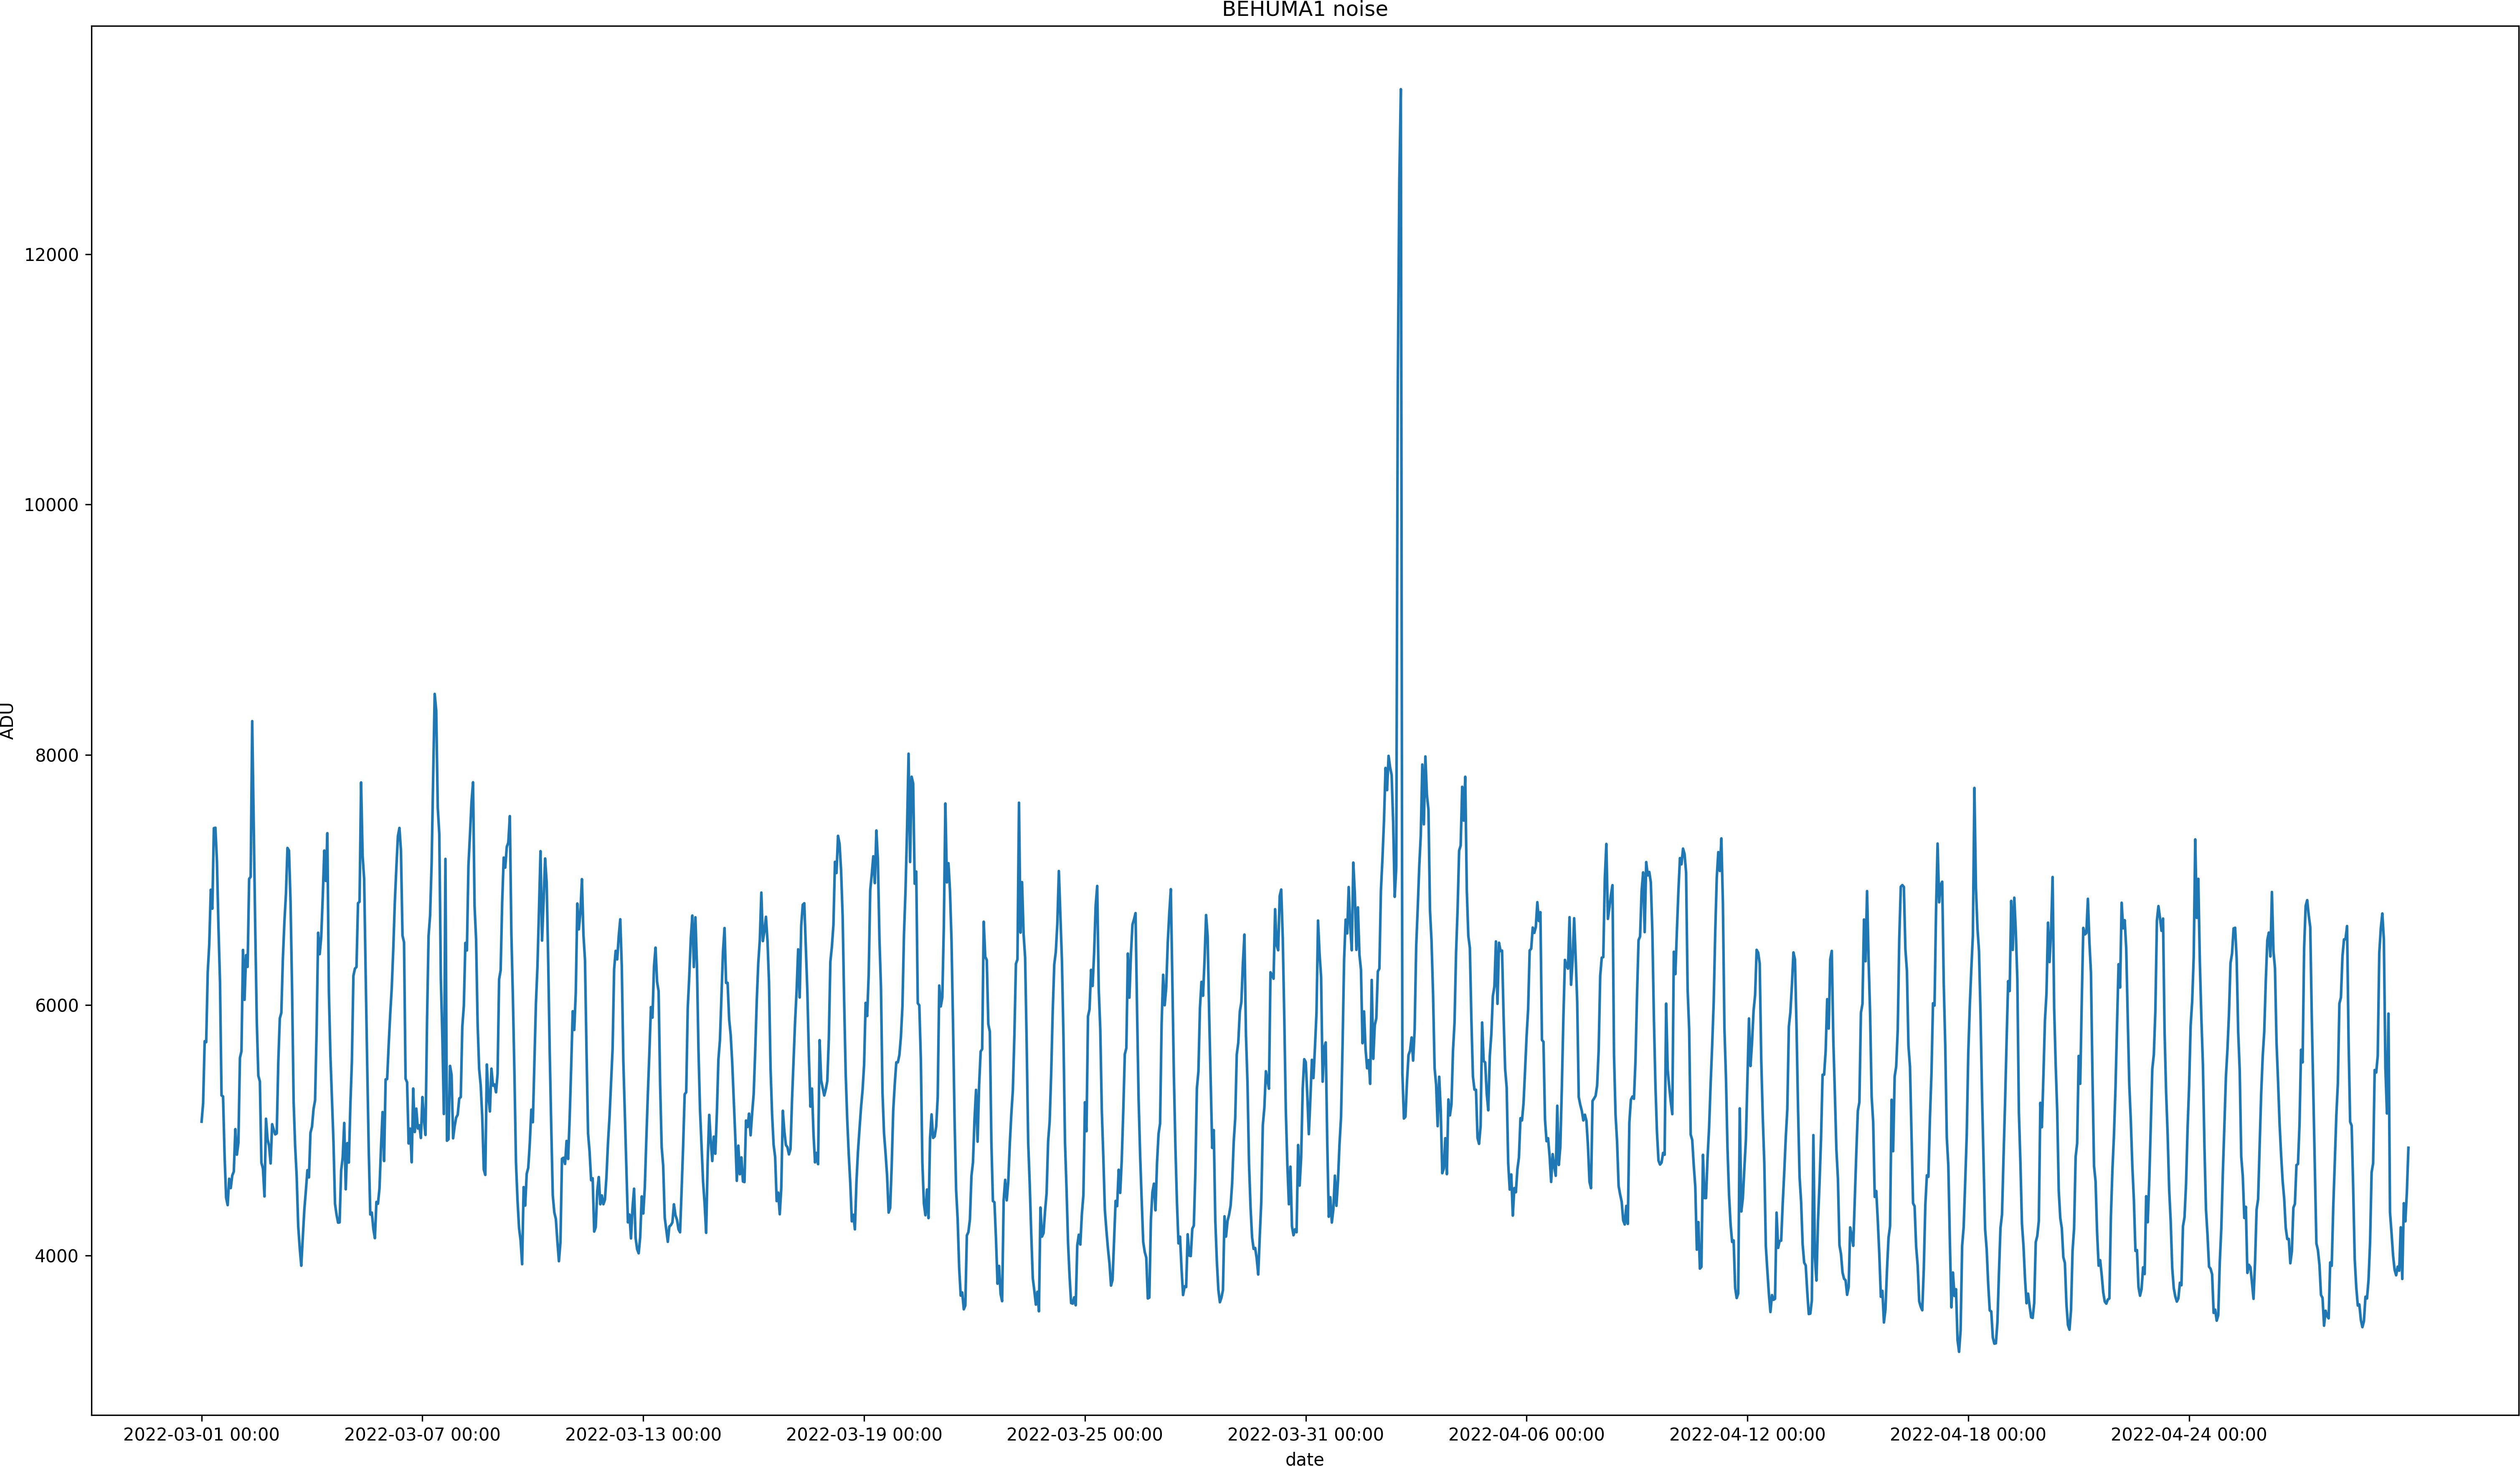
\includegraphics[scale=0.225]{page_garde.png}\\
        \vspace{0.14cm}
        \textit{2021-2022}
    \end{center}



    \vspace*{\stretch{2.0}}
\end{titlepage}

\section*{Remerciements}
\begin{remerciements}
    Je tiens tout d'abord à remercier toutes les personnes qui m'ont aidé à réaliser ce projet de fin d'études.\\
    \par
    En commençant par mon professeur rapporteur, à qui j'ai pu poser mes questions en cas de besoin et qui s'est assuré que tout se passe bien tout au long du projet.\\
    \par
    Ensuite, je voudrai remercier Mr Hervé Lamy pour avoir proposé ce sujet de fin d'études, mais également pour m'avoir expliqué, de façon claire et précise, toutes les notions qui nécessitaient des explications.\\
    \par
    Je tiens également à remercier Mrs Antoine Calegaro et Michel Anciaux, qui m'ont guidé quand c'était nécessaire et qui m'ont conseillé durant le projet de fin d'études.\\
    \par
    Enfin, je voudrais exprimer ma reconnaissance envers toutes les personnes qui m'ont conseillé sur, et ont relu ce rapport de projet de fin d'études.
\end{remerciements}

\newpage

\tableofcontents

\newpage

\section{Introduction}

\subsection{Le projet BRAMS}

Lancé en 2010 par Monsieur Hervé Lamy à l'Institut Royal d'Aéronomie Spatiale de Belgique, le projet BRAMS (Belgian RAdio Meteor Stations) à pour but de collecter et stocker des données relatives à des objets rentrant dans l'atmosphère belge et, plus précisément, des météores.
Ces données pourront ensuite être analysés afin de retrouver la trajectoire, la vitesse ou encore la masse d'un ou de plusieurs météores.\\

\subsubsection{Le Réseau BRAMS}

Afin d'accomplir ce but, le projet BRAMS dispose d'un réseau de stations nommé le réseau BRAMS.
Ce réseau est composé d'un ensemble de quarante-deux stations émettrices, situées en Belgique ou dans les pays avoisinants, et d'un émetteur dédié situé à Dourbes, dans le sud de la Belgique.\\
\\
Il existe 2 types de station de réception :
\begin{itemize}
    \item Il y a d'abord les stations avec des récepteurs Icom IC-R75, que j'apellerai les récepteurs ICOM dans ce document.
          Ce sont les premières stations réceptrices mises en service pour le réseau BRAMS.
          Actuellement, ces stations ne sont plus utilisées suite à l'arrêt de la commercialisation du récepteur Icom IC-R75.
          De plus, une variation de température pouvait causer une légère déstabilisation en fréquence.
    \item C'est alors que les stations utilisant le récepteur RSP 2 ont été développés.
          Ces stations n'éliminaient pas seulement en grande partie les problèmes des anciennes stations, mais sont également plus compacts et plus faciles à installer.
          Une image des stations RSP 2 peut être trouvé à la figure 1.
\end{itemize}

\begin{figure}[t]
    \begin{center}
        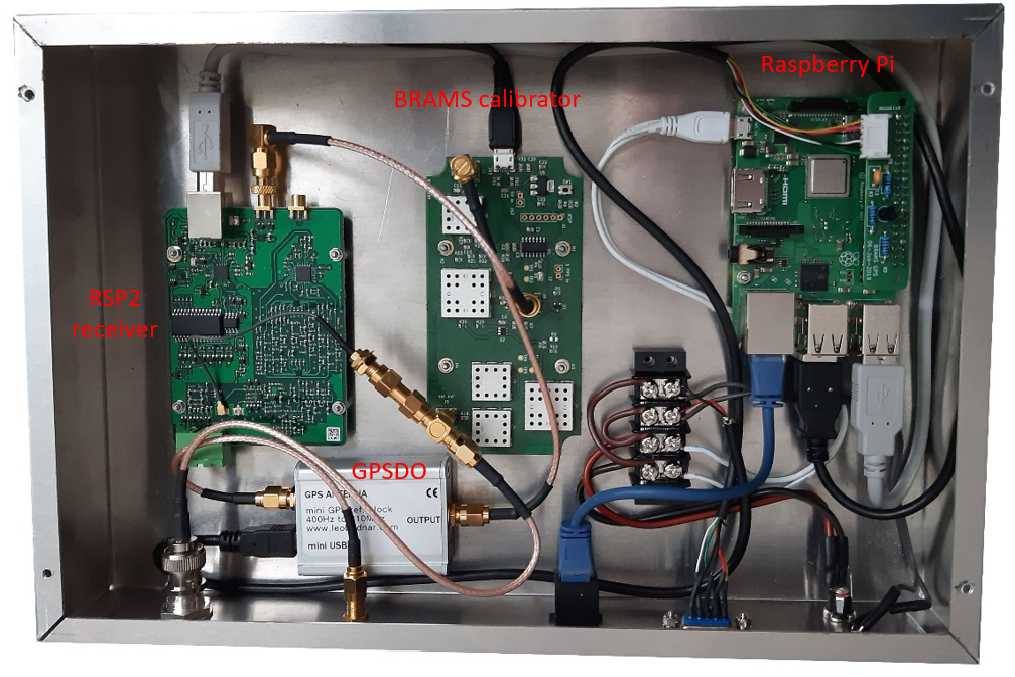
\includegraphics[scale=0.58]{RPS2.png}
        \caption{Station RSP 2 du réseau BRAMS}
    \end{center}
\end{figure}

\subsubsection{Le Format WAV}

Le format de fichier WAV (Waveform Audio File) est un format destiné au stockage de signal audio développé par Microsoft et IBM.
Il est construit conformément au RIFF (Ressource Interchange File Format) ce qui veut dire que le fichier est organisé en blocs de données, aussi nommés des "chunks" ou "data chunks".\\
\\
Chaque bloc de données dispose d'un ID codé sur 4 octets, qui représente souvent un mot de 4 lettres.
Suit ensuite le champ "ChunkSize" indiquant la taille des données à venir dans l'ensemble du fichier, codé également sur 4 octets.
Cette valeur exclut donc les champs "ID" et "ChunkSize" ainsi que la taille de tous les éventuels blocs de données venant avant le bloc courant.
Après ces 2 champs, on est libre de rajouter le nombre de champs que l'on souhaite, avec la taille en octets que l'on souhaite.\\
\\
Pour un fichier WAV, on retrouve typiquement 3 blocs de données.
On retrouve premièrement le bloc "RIFF" qui contient la taille de l'entièreté du fichier moins 8 octets (4 octets du champ "ID" et 4 octets du champ "ChunkSize") suivi du champ indiquant le format du fichier.
Dans le cas du fichier WAV, ce dernier contient les quatre lettres "WAVE".\\
\\
Le deuxième bloc contenu dans un fichier WAV ordinaire contient toutes les données techniques des données.
On y trouve notamment la fréquence d'échantillonnage, le nombre de pistes audio ou encore le nombre d'octets par secondes.\\
\\
Vient enfin le bloc principal du fichier : le bloc de données.
C'est dans ce bloc que se trouvent les données audio brutes.
La taille de ce bloc varie bien-entendu selon les caractéristiques techniques des données audio (longueur, fréquence d'échantillonnage, nombre de pistes, etc.).\\
\\
Une chose à noter à propos des fichiers WAV est que leur structure offre une grande flexibilité.
En effet, elle permet non-seulement de lire et interpréter les fichiers facilement, mais également de rajouter des blocs de données personnalisés sans corrompre les autres données.\\
\\
La figure 2 montre la structure d'un fichier WAV ordinaire.

\begin{figure}[t]
    \begin{center}
        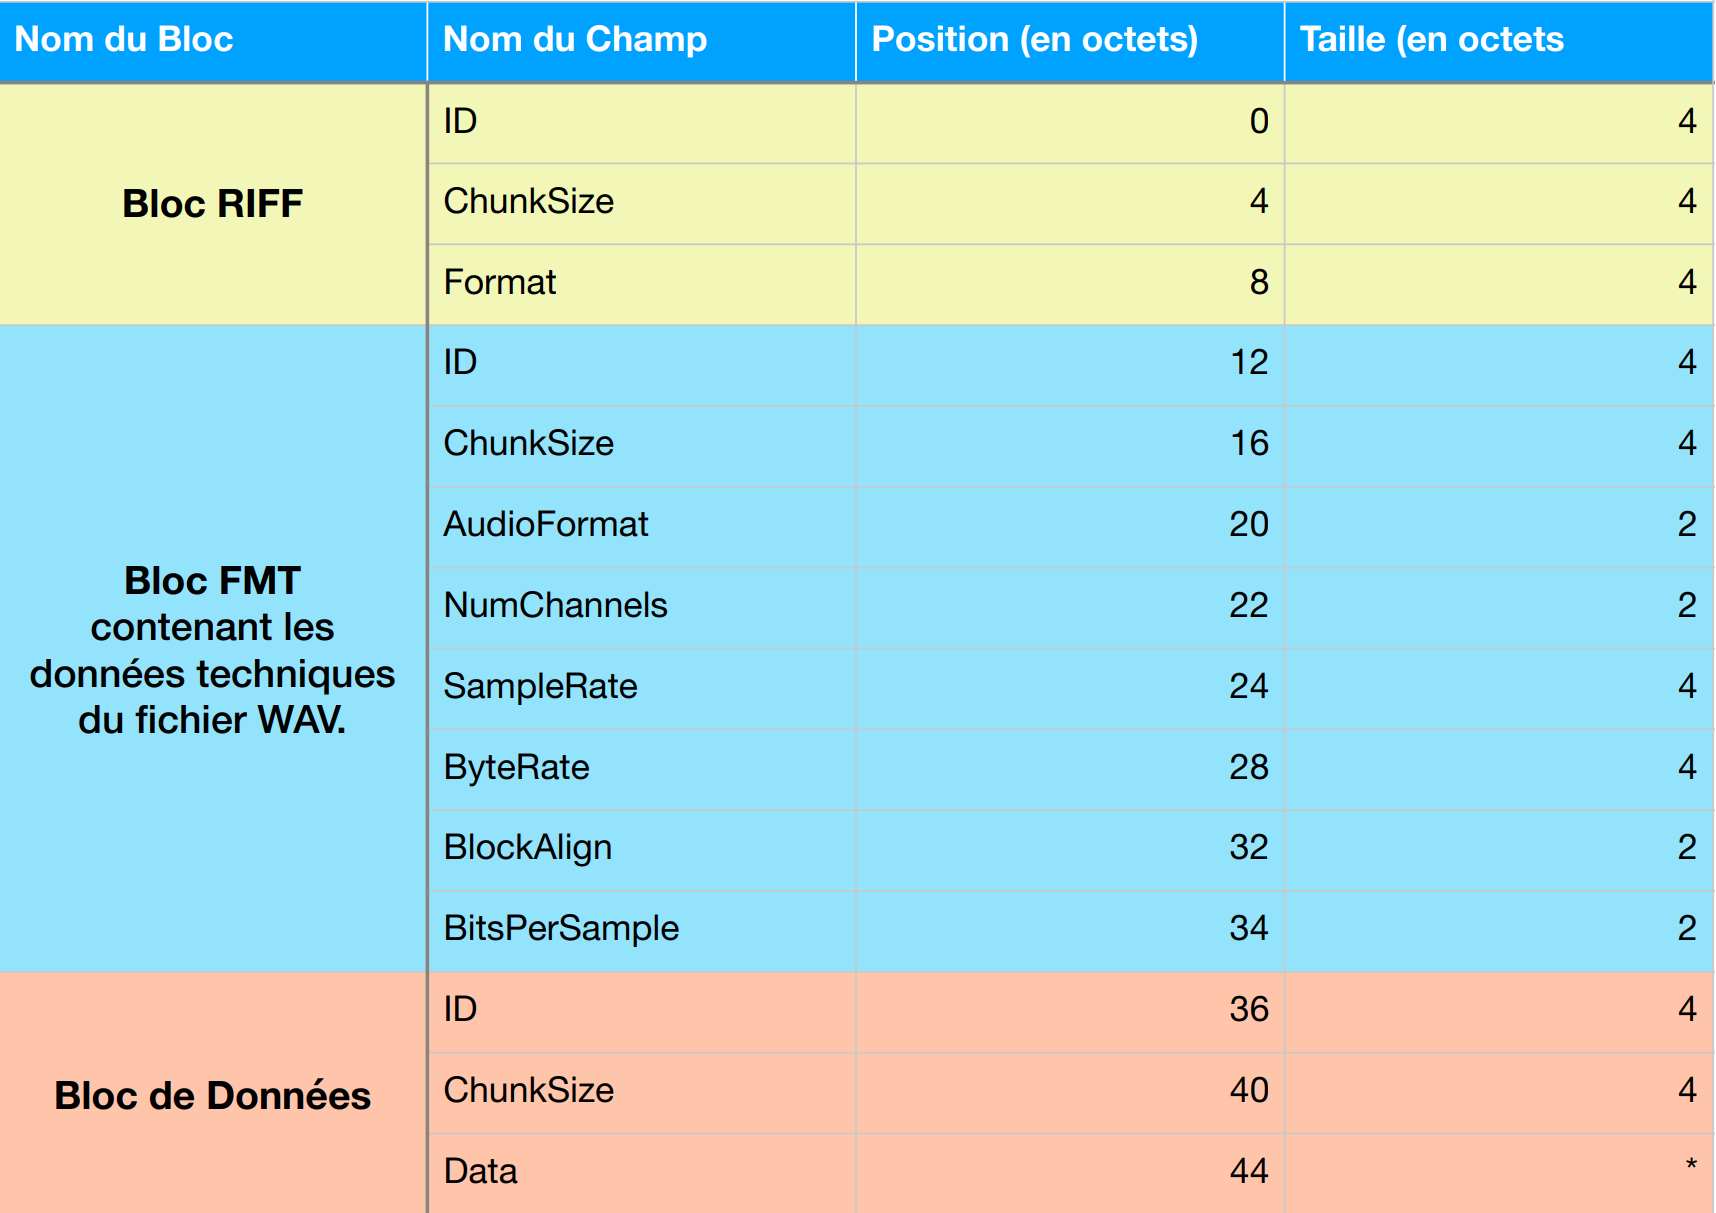
\includegraphics[scale=0.2]{Screenshot from 2022-05-22 22-49-39.png}
        \caption{Structure d'un fichier WAV ordinaire}
    \end{center}
\end{figure}

\newpage

\subsubsection{La Réflexion Spéculaire}

Pour comprendre le fonctionnement du réseau BRAMS, la première chose à savoir est : lorsqu'un météore passe dans l'atmosphère, il laisse derrière lui une trainée ionisée.
Cette trainée à la propriété de réfléchir les ondes radio.
Dans la plus grande partie des cas cette réflexion se fait en un seul point le long de la trajectoire, phénomène qui s'appelle la réflexion spéculaire (illustré à la figure 1).
La position de ce point, nommé le point de réflexion spéculaire, dépend notamment du positionnement de l'émetteur, du positionnement du récepteur et de la trajectoire du météore.\\
\\
Pour exploiter le phénomène de la réflexion spéculaire et réussir à détecter les météores à l'aide d'ondes radios, le réseau BRAMS fonctionne de la façon suivante :
\begin{enumerate}
    \item Un émetteur, situé à Dourbes, transmet de façon continue un signal à une fréquence de 49.97 MHz.
          Ce signal est émis en direction du ciel et peut être réfléchi sur des trainées ionisées dans le sillage des météores.
    \item Lorsque le signal est réfléchi, il peut être détecté par une ou plusieurs stations réceptrices faisant partie du réseau BRAMS.
          Un signal calibreur est alors additionné au signal venant du ciel.
          Ce signal est injecté à 49.9705 MHz, c'est-à-dire 500 Hz plus haut que le signal direct.
          Il dispose d'une amplitude fixe et sert de référence d'amplitude pour le reste du signal.
          La station réceptrice décale ensuite le signal direct de 49.97 MHz vers une fréquence de 1 kHz.
    \item Ensuite, la station réceptrice enregistre l'ensemble du signal dans un fichier audio de type WAV.
          Le signal est échantillonné à une fréquence de 5512,5 Hz pour les stations ICOM et 6048 Hz pour les stations RSP2.
          Si tout se passe bien, un fichier est généré toutes les cinq minutes et chaque fichier devrait commencer et terminer à un temps prédéfini (par exemple : 16 h 00 à 16 h 05, 16 h 05 à 16 h 10, etc.).
    \item Tous les fichiers générés par les stations réceptrices sont envoyés à intervalle régulier aux serveurs utilisés pour le projet BRAMS par internet.
    \item Une fois sur le serveur, les fichiers WAV sont archivés, manipulés et étudiés par les scientifiques du projet BRAMS afin d'en extraire les informations utiles.
\end{enumerate}

\subsubsection{Les Données BRAMS}

Un fichier WAV venant d'une station réceptrice contient donc le signal capté par l'antenne ensemble avec un signal calibreur.
Il est composé d'une seule piste audio, échantillonnée à une fréquence de 5512.5 Hz ou 6048 Hz.
Cette fréquence permet d'enregistrer des données dans une bande de fréquences allant jusqu'à 2756.25 Hz ou 3024 Hz (ou la moitié de la fréquence d'échantillonnage), selon le théorème de Nyquist.
Sachant que les échos de météores apparaissent typiquement dans une bande de fréquence de 100 Hz autour du signal de l'émetteur à 1000 Hz, cette bande de fréquence couvre l'ensemble des signaux utiles à l'étude des météores.\\
\\
À chaque fichier WAV est rajouté un bloc de données (data chunk) dans lequel sont insérés quelques informations relatives à la station de réception, la station émettrice, le signal GPS\footnote{Global Positioning System} ou encore, la fréquence d'échantillonnage.



\end{document}